\chapter{Architettura del prodotto}\label{ArchitetturaDelProdotto}

\section{Descrizione generale}
In fase di progettazione, il gruppo \textit{Jawa Druids} ha deciso di suddividere la modellazione architetturale di \textit{Gathering-Detection-Platform} in tre distinti moduli, tutti indipendenti tra loro.
Il primo modulo si occupa solamente di leggere, tramite file JSON$_G$, tutte le webcam disponibili per poi effettuare il riconoscimento persone tramite i frame scaricati. Successivamente i dati estrapolati verranno invitati al database.
Il secondo modulo, il machine-learning$_G$, si occupa di recuperare questi dati dal database per lavorarli producendo predizioni per le ore future.
Infine il terzo modulo, la web-app$_G$ vera e propria, si occuperà di rappresentare graficamente i dati all'interno del database mediante una heat-map$_G$ e farli visualizzare all'utente.

\section{Architettura Acquisition}\label{ArchitetturaDelProdottoAcquisition}
L'architettura riguardante il modulo di acquisizione, ovvero il primo modulo del software, è molto semplice ed intuitiva.
Non vi è alcuna classe e si basa su una programmazione procedurale.
Nel \textit{detect.py}, ovvero lo script principale del modulo, vengono richiamate le funzioni, in maniera sequenziale, per scaricare e manipolare i dati delle webcam.
La scelta dell'utilizzo di un paradigma procedurale risiede nel fatto che la creazione di oggetti e il loro utilizzo risultavano, nell'insieme, più complicati mentre chiamando delle semplici funzioni esterne il programma risultava più leggibile ed efficiente.
Gli unici oggetti presenti in \textit{detect.py} sono quelli di tipo \textit{data}, necessari per la giusta esecuzione dello script.
Di seguito vengono riportati i diagrammi relativi all'\textit{attività} e di \textit{package}.
%Inserire
%Grafici

\section{Architettura Prediction}\label{ArchitetturaDelProdottoPrediction}
L'architettura del modulo del machine-learning si può semplificare ad un modulo unico con all'interno i metodi necessari per prelevare dati dal database per generare delle predizioni ed archiviarle nel database.
Non necessita classi interne in quanto svolge esclusivamente operazioni funzionali. Per generare le predizioni il modulo svolge delle operazioni sequenziali:
\begin{enumerate}
	\item prelevo i dati all'interno del database;
	\item controllo dei dati per eliminare le informazioni che possono inquinare le predizioni;
	\item definisco il modello della predizione;
	\item alleno il modello con i dati prelevati e controllati;
	\item creo un set di dati da predire e utilizzando il modello ricavo il risultato;
	\item archivio il risultato nel database.
\end{enumerate}
%Inserire
%Grafici
\subsection{Diagrammi dei package}
\begin{center}
	\begin{figure}[H]
		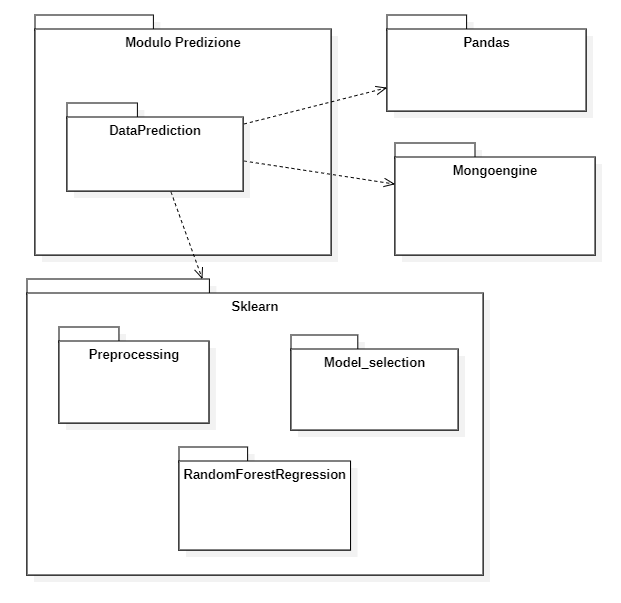
\includegraphics{../immagini/diag_PB/diag_pack_pred.png}
		\caption{Diagramma dei package del modulo della predizione}
	\end{figure}
\end{center}

\section{Architettura Web-App}\label{ArchitetturaDelProdottoWebApp}
Per il modulo relativo al front-end$_G$, si è deciso di utilizzare il pattern \textit{Model-View-Controller}(MVC).
Questa scelta è dovuta al fatto che, essendo la web-app sviluppata con spring, il pattern è quello che più si adatta alla tipologia sia di modellazione sia di scopo.
Lo scambio di dati tra fron-end e back-end avviene attraverso il pattern architetturale REST. Si è deciso questo pattern per avere un oggetto di scambio tra le due parti unico strutturalmente e quindi non è essere vincolato dalla struttura presente nel database.
Questo permette di aumentare la portabilità dell'applicazione web potendo applicare il back-end, possibilmente, a diversi front-end. Le richieste che il front-end effettua al back-end sono HTTP Request GET, quindi sono sempre richieste di visione di informazioni per poi essere utilizzate per aggiornare la parte grafica visibile dal client.
%Inserire
%Grafici
